\documentclass[a4paper, 12pt]{report}
\usepackage[utf8]{inputenc}
\usepackage[T1]{fontenc}

\usepackage{xcolor}
\usepackage{afterpage}

\usepackage{relsize}
\usepackage{moresize}

\usepackage{graphicx}
\usepackage{geometry}

\usepackage{hyperref}
\usepackage{apacite}

\usepackage{amsmath}
\usepackage{amssymb}

\usepackage{caption}
\usepackage{subcaption}

\usepackage{algorithm}
\usepackage{algpseudocode}

\algrenewcommand\algorithmicrequire{\textbf{Input:}}
\algrenewcommand\algorithmicensure{\textbf{Output:}}

\newcommand{\approxtext}[1]{\ensuremath{\stackrel{\text{#1}}{\approx}}}

\setcounter{secnumdepth}{3}
\setcounter{tocdepth}{3}

% [CHANGE] The title of your thesis. If your thesis has a subtitle, then this
% should appear right below the main title, in a smaller font.
\newcommand{\theTitle}{The first sentence \\
\vspace{0.5em}
the second sentence}
\newcommand{\theSubTitle}{a smaller subtitle}


% [CHANGE] Your full name. In case of multiple names, you can include their
% initials as well, e.g. "Robin G.J. van Achteren".
\newcommand{\theAuthor}{Dewi E. Timman}

% [CHANGE] Your student ID, as this has been assigned to you by the UvA
% administration.
\newcommand{\theStudentID}{12419273}

% [CHANGE] The name of your supervisor(s). Include the titles of your supervisor(s),
% as well as the initials for *all* of his/her first names.
\newcommand{\theSupervisor}{Dr. V. Niculae} % Dr. Ing. L. Dorst

% [CHANGE] The address of the institute at which your supervisor is working.
% Be sure to include (1) institute (is appropriate), (2) faculty (if
% appropriate), (3) organisation name, (4) organisation address (2 lines).
\newcommand{\theInstitute}{
Informatics Institute \\ %Institute for Logic, Language and Computation
Faculty of Science\\
University of Amsterdam\\
Science Park 900 \\ 
1098 XH Amsterdam 
}

% [CHANGE] The semester in which you started your thesis.
\newcommand{\theDate}{Semester 1, 2023-2024}

\begin{document}
\pagestyle{empty}
\begin{center}

\vspace{2.5cm}


\begin{Huge}
% see definition at beginning of document
\theTitle
\end{Huge} \\

\vspace{0.5 cm}

\begin{Large}
\theSubTitle
\end{Large}

\vspace{1.5cm}

% see definition at beginning of document
\theAuthor\\
% see definition at beginning of document
\theStudentID

\vspace{1.5cm}

% [DO NOT CHANGE]
Bachelor thesis\\
Credits: 18 EC

\vspace{0.5cm}

% [DO NOT CHANGE] The name of the educational programme.
Bachelor \textit{Kunstmatige Intelligentie} \\
\vspace{0.25cm}

\includegraphics[width=0.075\paperwidth]{figs/uva_logo} \\
\vspace{0.1cm}

% [DO NOT CHANGE] The address of the educational programme.
University of Amsterdam\\
Faculty of Science\\
Science Park 900\\
1098 XH Amsterdam

\vspace{2cm}

\emph{Supervisor}\\

% see definition at beginning of document
\theSupervisor

\vspace{0.25cm}

% see definition at beginning of document
\theInstitute

\vspace{1.0cm}

% see definition at beginning of document
\theDate

\end{center}
\newpage

\pagenumbering{arabic}
\setcounter{page}{1}
\pagestyle{plain} 

\chapter*{Abstract}
To make tasks more efficient, an autocomplete system can predict a full sentences from a partial sentence.
To do this, the system needs to be as accurate and efficient (as few tokens as possible) as possible. 
In order to train such an autocomplete system, an encoder decoder model is made. 
The encoder extracts keywords from a sentence, and the decoder tries to predict the full sentence from these keywords.
First, the model of \shortciteA{autocomplete} was replicated. 
This work was one of the first to extract keywords from across the full sentence instead of the first or the last few words. 
However, this was done in an unstructured manner. 
Since human language is structured, this calls for a structured manner of extracting keywords. 
Therefore, the second model in this paper is a structured model. 
In order to achieve this, the encoder was adjusted to extract keywords using a segmentation model. 
With the help of dynamic programming algorithms the keywords could be extracted resulting in \textcolor{orange}{\dots.}

\textcolor{red}{TODO:\begin{enumerate}
    \item add results
    \item add conclusion
    \item add discussion
\end{enumerate}}

\paragraph{Keywords:} segmentation, dynamic programming, autocompletion, autoencoder, communication, latent variables

\tableofcontents

\chapter{Introduction}
% What am I researching? bruggetje met taal
% \begin{itemize}
%     \item keywords $\rightarrow$ sentence
%     \item efficient, accurate, interpretable
%     \item this research: segmentation model more effective, natural, flexible than a bit mask?
% \end{itemize}

What if machines can read our mind? 
If we can give a machine a few keywords and let the machine generate a sentence from these keywords, our lives would become more productive and efficient. 
This is what autocomplete systems are trying to achieve. 
\textcolor{orange}{The way in which we choose the keywords is also important. 
Taking just the first or the last few words of a sentence as keywords usually does not capture the full meaning of the sentence.} 
For example, if someone want to capture the meaning of \textit{'I live in Amsterdam'} in a few keywords, the words \textit{'live Amsterdam'} would probably be choosen. 
Thus, the keywords come from multiple places in the sentence. 
Therefore, autocomplete systems need to use more complex models to be more efficient and accurate. 

\section{Literature review}
% TODO:delete

\subsection{Autocomplete communication game}

\begin{figure}
    \centering
    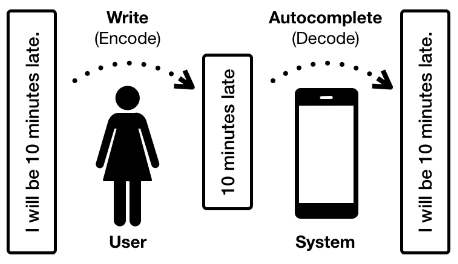
\includegraphics[width=.5\linewidth]{figs/autocomplete_game.png}
    \caption{schematic overview of the communication game. Figure from \protect\shortciteA{autocomplete}.}
    \label{fig:autocomplete}
\end{figure}

The same autocomplete communication game is considered as in \shortciteA{autocomplete}. In this game, a human (called user) encodes a sentence into keywords. 
These keywords are then decoded by a machine (called system) to retrieve the full, initial sentence. 
A schematic overview is given in figure \ref{fig:autocomplete}. 
The communication game is succesfull if the retrieved sentence is the same as the initial sentence. 

More formally, a target sentence $x=(x_1, \dots, x_m)$ is communicated by a user through the keywords $z=(z_1, \dots, z_n)$. 
Note that $z$ is a subsequence of $x$. 
The system then tries to retrieve the target sentence by decoding the keywords. 
The target sentence is described by the keywords using encoding strategy $q_{\alpha}(z | x)$ and the system decodes the keywords by using decoding strategy $p_{\beta}(x|z)$. 

For a model to be efficient, the number of keywords needs to be as low as possible. 
In addition, for a model to be accurate, the probability of reconstructing $x$ from $z$ needs to be as high as possible. 
Therefore, a cost and a loss, respectively, can be defined:
\begin{equation}
    \label{eq:cost}
    \text{cost}(x,\alpha) = \mathbb{E}_{q_{\alpha}(z|x)} [\text{length}(z)]
\end{equation}
\begin{equation}
    \label{eq:loss}
    \text{loss}(x,\alpha,\beta) = \mathbb{E}_{q_{\alpha}(z|x)} [-\log p_{\beta}(x|z)]
\end{equation}

\subsection{Segmentation model}
\label{sec:segmentation}
% Why does a segmentation model work?

\paragraph{General idea.}
If there is a rod of length $n$ and we can cut this rod at every marker, how can we best find the maximal total value of the resulting pieces?
This is called the rod cutting problem.
The segmentation model gives a solution to the rot cutting problem. 
The segmentation model takes the scores of all pieces of the rod, called segments. 
Those segments can be of length 1, 2 or even $n$. 
With these scores, the model determines what the best possible segmentation is. 
To find the best segmentation and the probability of a segmentation, the model makes use of dynamic programming algorithms such as the Viterbi algorithm \shortcite{Viterbi} and the forward algorithm.
The segmentation model is essentially a simpler version of a hidden semi-Markov model \shortcite{hsmms}. 

\paragraph{Segmentation model for text.}
So how does the segmentation model work for text? 
If we have a sentence, e.g. \textit{'I will be late'}, we can use fencepost indexing to represent a sentence as a rod which can be cut at the fenceposts (see also figure \ref{fig:fencepost}).
The fenceposts can also represent nodes in a directed acyclic graph (DAG). 
We can then draw edges between those nodes that represent segments. 
Those segments can be seen as (groups of) words. 
In figure \ref{fig:dag}, a DAG can be seen in which all the possible segments are showed. 
In the case of the autocomplete communication model described before, a segment is either kept or not.
Therefore, we can have one edge representing 'keep' and one representing 'do not keep', resulting in figure \ref{fig:dag2}.
If the pink edges are taken as 'do not keep' and the blue ones as 'keep', two possible segmentations can be seen in figure \ref{fig:segmentation} and \ref{fig:segmentation2}. 
Both segmentations result in the keywords \textit{'will be late'}. 

The score of a segmentation can be calculated by summing up all scores of its segments.
The assigned score of a segment can visualized as a score matrix $A$ and has size $(m+1) \times (m+1)$. 
A segment, e.g. segment $i-j$, only has a score if it goes to a node further in the sequence, i.e. $i < j$.
Therefore, only the upper triangle of the matrix is used. 
This is denoted in figure \ref{fig:matrixA} by the gray squares.
The scores of the segmentations can then be used to calculate probabilities and to sample from a distribution over segments.

\begin{figure}
    \centering
    \begin{subfigure}[b]{0.45\textwidth}
        \centering
        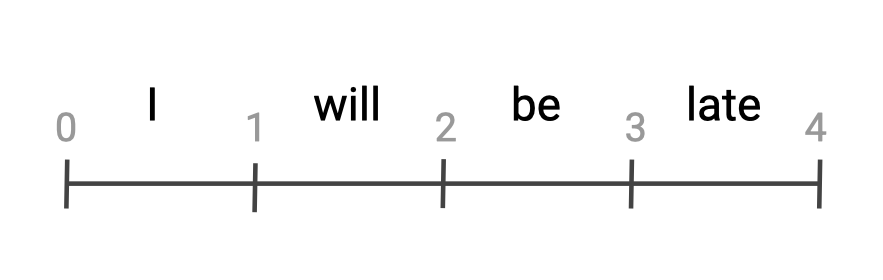
\includegraphics[width=\textwidth]{figs/fencepost.png}
        \caption{Fencepost indexing}
        \label{fig:fencepost}
    \end{subfigure}
    \hfill
    \begin{subfigure}[b]{0.45\textwidth}
        \centering
        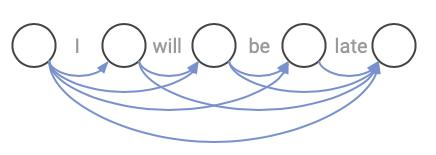
\includegraphics[width=\textwidth]{figs/segmentation1.jpeg}
        \caption{Possible segments in a DAG}
        \label{fig:dag}
    \end{subfigure}
    \hfill
    \begin{subfigure}[b]{0.45\textwidth}
        \centering
        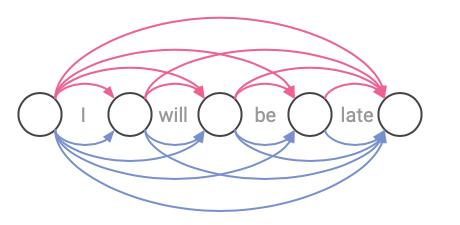
\includegraphics[width=\textwidth]{figs/segmentation2.jpeg}
        \caption{Possible segments in a DAG when each segment can either be true or false}
        \label{fig:dag2}
    \end{subfigure}
    \hfill
    \begin{subfigure}[b]{0.45\textwidth}
        \centering
        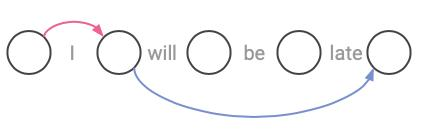
\includegraphics[width=\textwidth]{figs/segmentation3.jpeg}
        \caption{A possible segmentation}
        \label{fig:segmentation}
    \end{subfigure}
    \hfill
    \begin{subfigure}[b]{0.45\textwidth}
        \centering
        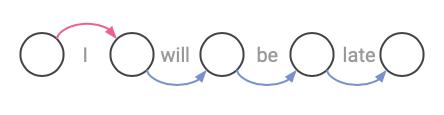
\includegraphics[width=\textwidth]{figs/segmentation4.jpeg}
        \caption{Another possible segmentation}
        \label{fig:segmentation2}
    \end{subfigure}
    \hfill
    \begin{subfigure}[b]{0.45\textwidth}
        \centering
        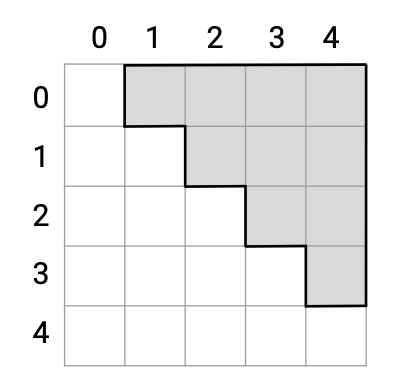
\includegraphics[width=0.6\textwidth]{figs/matrixA.png}
        \caption{Score matrix A}
        \label{fig:matrixA}
    \end{subfigure}
    \caption{Segmentation model}
    \label{fig:segmentation_model}
\end{figure}

\subsection{Structured latent variables}
A latent variable is an unobservable variable.
For these variables, there are no labels available. 
Therefore, it is not possible to use supervised learning on them. 
In the case of this model, we try to recover the full sentence by inferring what is a good mask.
The mask determines what words are good keywords and thus is a latent variable. 
In addition, the segmentation model makes this a structured variable. 

% Previous research on segmentations predicted a segmentation as output, rather than as a latent variable \shortcite{hsmms,conditionalRandomFields,kong2016segmentalrecurrentneuralnetworks}. 

\section{Current research}
% Gap
% Research question: To what extend can a segmentation model help by selecting keywords for an auto-complete communication game?
% TODO: check references - are they relevant?
% into account for what?

Previous research did not take structure into account \shortcite{Bar-YossefZiv2011Cqa,autocomplete,SvyatkovskiyAlexey2019PACC}.
Since language is structured, it makes sense to use a structured model as an autocomplete model. 
Furthermore, previous work has shown that the prediction of segmentations can lead to better results than models that do not explicitly represent segments \shortcite{kong2016segmentalrecurrentneuralnetworks,conditionalRandomFields}. 
Therefore, in this research, we look at how a latent segmentation model can be used to retrieve keywords from a sentence. 
The segmentation model will be implemented in the encoder of the encoder-decoder model in order to choose the best keywords from the sentence.

\chapter{Experiment 1 \\ Replication}
\label{ch:repl}
% TODO: check if lambda misses in control variate function
In the first experiment the autoencoder model from \shortciteA{autocomplete} was replicated. 

\section{Method}
To replicate the model, an encoder-decoder model was made. The encoder chooses which words to keep as keywords, and the decoder tries to retrieve the full sentence of the keywords. 

\subsection{Data}
\label{sec:data}
The same data was used as in \shortciteA{autocomplete}.
The data used to train the model consisted of 1K randomly sampled sentences from the Yelp restaurant reviews corpus \shortcite{data}.
Another 100 sentences were used to evaluate the model. 
The sentences had at most 16 tokens. 
The reviews were segmented into sentences following the same procedure as in \shortciteA{GuuKelvin2018GSbE}. 

The model of \shortciteA{autocomplete} also predicts capital letters and whitespaces. 
However, for English we can just assume that after every word a space is used. 
Therefore, the data was adjusted to leave out the characters for whitespaces. 
Something similar is also true for capital letters: usually these only occur at the start of a sentence or in names. 
It is thus not necessary to also predict capital letters. 

\subsection{Experimental Design}
The model used is an encoder-decoder model.
For a schematic overview, see figure \ref{fig:autocomplete}.
The encoder, using the encoding strategy $q_{\alpha}(z|x)$, takes as input a target sequence $x = (x_1, \dots, x_m)$ and outputs a sequence of keywords $z = (z_1, \dots, z_n)$.
The decoder, using the decoding strategy $p_{\beta}(x|z)$, then takes these keywords as input and outputs a predicted sequence $y = (y_1, \dots, y_k)$. 
The better the autoencoder works, the more likely it is that $x$ and $y$ are equal. 
Table \ref{tab:example} gives an example of a sentence, a possible mask and the keywords generated using that mask.

\begin{table}
    \centering
    \begin{tabular}{|cl|}
        \hline
        sentence & <sos> the vibe is urban modern . <eos> \\
        mask & $\quad$ 0 $\quad$ 0 $\quad$ 1 $\quad$ 0 $\quad$ 1 $\quad$ 1 $\quad$ 0 $\quad$ 0 \\
        keywords & vibe urban modern  \\
        \hline
    \end{tabular}
    \caption{Example sentence, mask and keywords}
    \label{tab:example}
\end{table}

\subsection{Model description}
\label{sec:model}
% TODO: add diagram?
\paragraph{Encoder.} 
The encoder embeds the tokens and uses a uni-directional LSTM \shortcite{LSTM} to score the tokens.
An additional linear layer followed by sigmoid function is used to determine the probability of keeping each token. 
From these probabilities, a mask is sampled from a Bernoulli distribution. 
Finally, the sequence of kept tokens and the log probability of the mask are returned.

\paragraph{Decoder.} 
The decoder itself is also an encoder-decoder model (the encoder of this model is referred to as encoder*).
The encoder* first embeds the tokens of the subsequence.
It then encodes the embedding using a bidirectional LSTM. 

The decoder decodes the full sentence. 
It therefore embeds the already decoded sequence (or just the <sos> symbol if there is none) into a 32-dimensional vector and concatenates the last hidden state of the encoder* to it. 
This embedding is the input for another uni-directional LSTM. 
Finally, the probability of the next word is calculated using global attention \shortcite{LuongAttention, bahdanau2016neuralmachinetranslationjointly} and the full sentence and its log probability are returned. 

During training, the decoder is given the keywords and at every step the model takes the correct word from the target sequence and calculates the probability of that sequence.
During evaluation, however, the decoder uses a greedy decoding strategy and thus takes the word with the highest probability as the next word. 
% TODO: <sos> anders verwoorden

\paragraph{Optimization.} 
The goal of the model is to be as efficient and accurate as possible. 
If equation \ref{eq:cost} and \ref{eq:loss} are merged and a parameter $\lambda$ is added to represent the trade-off between the two, the goal becomes the following:
\begin{equation}
    \label{eq:loss2}
    \min_{\alpha, \beta} \mathbb{E} [\text{cost}(x, \alpha)] + \lambda \cdot \mathbb{E}[\text{loss}(x, \alpha, \beta)].
\end{equation}
Here the expectation is taken over $x$. 
Since the gradients of equation \ref{eq:loss2} cannot be calculated, it is approximated with Monte Carlo.
The gradients can then be calculated as following (see appendix \ref{app:gradients} for the exact derivations):

\begin{equation}
    \label{eq:gradient_alpha}
    \nabla_\alpha F(x, z, \alpha, \beta) = \mathbb{E}_{q_{\alpha}(z|x)} [\nabla_{\alpha} \log q_{\alpha}(z|x) f(x, z, \beta)],
\end{equation}
\begin{equation}
    \label{eq:gradient_beta}
    \nabla_\beta F(x, z, \alpha, \beta) = \mathbb{E}_{q_{\alpha}(z|x)} [\nabla_{\beta} f (x, z, \beta)].
\end{equation}
Where, $f$ and the score function estimator (SFE) $F$ (and its Monte Carlo approximation) are:
\begin{equation}
    \label{eq:f}
    f(x, z, \beta) = \text{length}(z) + \lambda \cdot (-\log p_{\beta}(x|z)),
\end{equation}
\begin{equation}
    \label{eq:F}
    F (\alpha, \beta) = \mathbb{E}_{q_{\alpha}(z|x)} [f(x, z, \beta)],
\end{equation}
\begin{equation}
    \label{eq:F_approx}
    F (\alpha, \beta) \approxtext{M.C.} \frac{1}{M} \sum_i f (x, z^{(i)}, \beta).
\end{equation}
Here $M$ is the amount of samples drawn from $q_{\alpha}(z|x)$.

\subsection{Hyperparameters}
\label{sec:hyper}
During training, the sentences start with a <sos> symbol and end with a <eos> symbol.
During evaluation of the model, those symbols are removed.

The model is implemented using PyTorch \shortcite{pytorch}.
After each token is embedded, a ReLu is used with a dropout rate of 10\% during training to prevent overfitting. 
The hidden dimensions of the LSTM layers are all 32. 
To optimize the model an Adam optimizer \shortcite{adam} is used with a learning rate of 0.01. 
Multiple models were trained for 10 epochs with different values for $\lambda$.

\subsection{Optimizations}
\label{sec:optimizations}
To let the model predict better results faster, a few optimizations were done.

\paragraph{Copy mechanism.} The copy mechanism \shortcite{copyMechanism} in the decoder determines if it wants to copy the current token or wants to generate a new token. 
It therefore calculates the probability of the new word as following:
\begin{equation}
    p(w) = (1 - p_{\text{gen}}) \cdot p_{\text{copy}}(w) + p_{\text{gen}} \cdot p_{\text{word}}(w).
\end{equation}
For the calculation of the probability of the to be copied word, $p_{\text{copy}}(w)$, the global attention mechanism from the decoder is used. 
To calculate the probability of generating a new word, $p_{\text{gen}}$, the last hidden decoder state, the attention mechanism and the token embedding of the new to generated word are used in a linear layer followed by a sigmoid.
$p_{\text{word}}(w)$ is the probability of the to be generated word if a word is being generated. 

\paragraph{Adjusted vocabulary.} The model makes a vocabulary to translate words to numbers. 
During the evaluation of the model, a lot of unknown tokens were encountered.
This was due to words that were not present in the training set but were in the validation set. 
To solve this problem, the vocabulary was made using the whole dataset, instead of just the training set. 
\shortciteA{autocomplete} used the copy mechanism and a dynamic vocabulary for this, but for the task at hand and the amount of data this also works.

\paragraph{Variance reduction.} Because of the use of an SFE the gradient can be more prone to noise \shortcite{niculae2023discretelatentstructureneural}.
To solve this problem, its variance can be reduced in a couple of ways. 
One of those solutions is to sample a second subsentence in the encoder \shortcite{RennieStevenJ2017SSTf}. 
With this second subsentence, $f(x, z', \beta)$ can be determined, and the loss can be updated as following:
\begin{equation}
    \mathbb{E}_{q_{\alpha}(z|x)} [\nabla_w \log q_{\alpha}(z|x) \cdot (f(x, z, \beta)-f(x, z', \beta))] + \mathbb{E}_{q_{\alpha}(z|x)} [\nabla_w f(x, z, \beta)],
\end{equation}
where $w$ is a parameter (i.e. either $\alpha$ or $\beta$). Note that the gradient is not changed when subtracting $f(x, z', \beta)$ from $f(x, z, \beta)$ since it can be seen as constant because it is independent of $z$.


\chapter{Experiment 2 \\ Segmentation Model}
In the second experiment, the model from chapter \ref{ch:repl} is expanded with a segmentation model. 

\section{Method}
An autoencoder model is made in which the encoder uses a segmentation model to choose the sequence of keywords $z$.
The same data was used as described in section \ref{sec:data}.

\subsection{Score matrix}
In order for this model to work, it needs a score tensor, $\boldsymbol{A}$.
This tensor consists of two upper triangle matrices of $(m+1) \times (m+1)$, called $A_0$ and $A_1$.
Both matrices represent the score of segments in the DAG made for each sentence as described in \ref{sec:segmentation}. 
The matrix $A_1$ represents the scores for when the segment is true, and $A_0$ for when the segment is false.
The matrix $A_0$ consists of only zeros to simplify the model.

To construct $A_1$, an embedding matrix $H$ with dimensions $m \times d$ is used.
Here $m$ is the amount of tokens in $x$ and $d$ the hidden dimension of the LSTM.
In addition, a weight matrix $W$ with dimensions $d \times d$ is used.
This weight matrix is learned by the encoder. 
Matrix $A_1$ is then calculated as following:
\begin{equation}
    A_{ij1} = h_i^T W h_j
\end{equation}
And more efficiently, with matrices:
\begin{equation}
    A_1 = H W H^T
\end{equation}
Note that the scores learned for $A_1$ can also be negative. 
Therefore, the model can prefer to leave out a segment when needed.

\subsection{Model description}
% TODO: logsumexp verwoorden
The same model as in section \ref{sec:model} was used. 
Only the encoder part was adjusted.
Instead of using an LSTM and a linear layer to score each token, the segmentation model is used.

\paragraph{Encoder.} The encoder embeds each token. 
It then uses a one-directional LSTM. 
The output of this LSTM is the matrix $H$, which is used to make the score matrix $a$, as described in the previous section. 
Then, using dynamic programming algorithms, a segmentation is sampled and its probability is calculated. 
As described in section \ref{sec:optimizations}, variance reduction is applied and thus also a second segmentation is sampled.
These segmentations are then converted into masks.

\paragraph{Dynamic programming.} To sample a segmentation, the forward filtering, backward sampling algorithm \shortcite{FFBS} was used.
This algorithm first calculates the logsumexp of all possible segmentations and then samples from this distribution.
Pseudocode for this algorithm can be found in algorithm \ref{alg:forward}.

To calculate the probability of the segmentation, the forward algorithm was used.
This algorithm calculates the logsumexp of all possible segmentations.
Pseudocode for this algorithm can be found in algorithm \ref{alg:ffbs}.
The logsumexp is then used in combination with the score of the segmentation (which can be calculated using a) to calculate the probability of the segmentation

\begin{algorithm}
\caption{Forward filtering, backward sampling algorithm}
\label{alg:ffbs}
\begin{algorithmic}
\Require score tensor $A$ with shape $(m+1) \times (m+1) \times 2$
\Ensure sampled segmentation
\State
\State $n \gets A.\text{shape[0]}$
\State $q_0 \gets 0$
\For{$i=1, \dots, n$}
    \State $q_i \gets \log \sum_{0 \leq j < i} (\exp (q_j + a_{ji0}) + \exp (q_j + a_{ji1}))$
\EndFor
\State
\State $y \gets []$
\State $i \gets n - 1$
\While{$i > 0$}
    \State sample $j < i$ and $k$ with probability $p_j \gets \exp (a_{ji0} + q_j - q_i) + \exp(a_{ji1} + q_j - q_i)$
    \State $y \gets (ji,k) \frown y$
    \State $i \gets j$
\EndWhile
\State
\State \Return $y$
\end{algorithmic}
\end{algorithm}

\begin{algorithm}
\caption{Forward algorithm}
\label{alg:forward}
\begin{algorithmic}
\Require score tensor $A$ with shape $(m+1) \times (m+1) \times 2$
\Ensure log-normalizer
\State
\State $n \gets A.\text{shape[0]}$
\State $q_0 \gets 0$
\For{$i=1, \dots, n$}
    \State $q_i \gets \log \sum_{0 \leq j < i} (\exp (q_j + a_{ji0}) + \exp (q_j + a_{ji1}))$
\EndFor
\State
\State \Return $q_n$
\end{algorithmic}
\end{algorithm}

% \subsection{Hyperparameters}
% The same hyperparameters as in section \ref{sec:hyper} were used.
% In addition, for the segmentation model ...
% TODO: describe parameters of the segmentation model

\section{Results}


\chapter{Results}

\chapter{Conclusion}
% repeat RQ + results
To see to what extent a segmentation model can help by selecting keywords in an autocomplete communication game, two different kinds of models were made and compared.
% summarize main findings
The results show no significant differences between the models.

% interpret findings
\paragraph{Accuracy.}
It is unusual for the accuracy to be higher on the validation set than on the training set. 
One possible reason for this can be an overlap between the two sets. 
However, after closer inspection this was not the case.
Other reasons can be the use of dropout or a small validation set. 

\paragraph{Cost.}
Both models have a high cost.
Therefore, the models find it hard to drop words. 
However, the unstructured model can have the tendency to keep all words in the sentence as keywords, especially when $\lambda$ is high.

\paragraph{Parameter $\boldsymbol{\lambda}$.}
For the segmentation model, the value of $\lambda$ does not seem to have any big difference on the accuracy, the cost and the training objective.
On the unstructured model, however, the higher the value of $\lambda$ the higher the cost, the accuracy and the training objective.
It is only logical for the accuracy to become higher when the cost increases, since more words are kept and therefore the model can just copy the keywords.
Consequently, the cost is part of the training objective and therefore the training objective will also be higher, especially when the value of $\lambda$ is high.
We can see that the model does drop more words with a higher $\lambda$, but it does not do so significantly. 
The training accuracy is higher than the validation accuracy, which can be a sign of overfitting. 
Figure \ref{fig:high_obj}, however, shows that the training objective does not share this phenomenon.


\paragraph{Training objective.}
The training objective does go down, but is still decreasing after 10 epochs for the unstructured model.
This can be a sign that the model still needs more training. 

\paragraph{Text analysis.}
When looking at the printed examples and comparing these to the cost, it seems that the lower the cost the more often the <sos> token is dropped. 

\chapter{Discussion}
% % main finding
No significant differences between the two models were found.

% comparison with previous research
\paragraph{Related work.}
This work is closely related to \shortciteA{autocomplete}. 
They share the same goal, namely to communicate as efficient and accurate as possible without losing interpretability. 
In order to do so, they propose two models and compare these to baseline models. 
Their linear model was replicated in chapter \ref{ch:repl}. 
In this work the same data was used as in their work.
However, due to computational resources our dataset was made considerably smaller and the prediction of capital letters and whitespaces was left out.
Moreover, the model was trained for fewer epochs (10 instead of 30) and with an embedding dimension of 32 instead of 300.

In their results they showed a figure similar to figure \ref{fig:acc_cost}.
For convenience, this figure is showed in figure \ref{fig:lee}.
In this work it was expected to find a similar trend. 
However, this was not found. 
This might be due to a smaller dataset and the smaller amount of training for our model.

We also notice that the values of $\lambda$ are significantly smaller than the ones found in figure \ref{fig:lee}.
This probably has to do with the lower embedding dimension and the smaller dataset.

\begin{figure}
    \centering
    \includegraphics[width=.5\textwidth]{figs/lee.png}
    \caption{Figure from \protect\shortciteA{autocomplete} comparing their two models on accuracy and cost. The Linear model is similar to our unstructured model.}
    \label{fig:lee}
\end{figure}

% implications
\paragraph{Implications.}
Communication between machines can take some time depending on how big the message is that the machines try to convey to each other.
When efficient communication schemes can be found, the message can first be compressed before sending it to another machine. 
In addition, with regard to humans, it can be more efficient for someone to write a text when only a few keywords are needed to write a full sentence. 
However, more future research is needed to find such a model.

% limitations
\paragraph{Limitations.}
As mentioned before, due to computational resources the models were a bit simpler than in \shortciteA{autocomplete}.
With more computational resources, more data could be used.
More data can mean a higher accuracy. 
Furthermore, the accuracy on the validation set is currently higher than on the training set. 
This could be due to the dropout. 
More data could solve this problem.
It should be noted, however, that in case more data is used, the model would benefit from a higher embedding dimension.

When looking at figure \ref{fig:obj}, we see that for the unstructured model the loss is still going down. 
Therefore, the models could benefit from longer training. 
Moreover, for the segmentation model the value of $\lambda$ does not seem to change a lot.
With more computational resources and time, the models could be trained longer and with different values of $\lambda$.

% unexpected results/patterns
\paragraph{Unexpected results.}
There were a few unexpected results.
First, during the training of the models it was observed that training on a GPU was not significantly faster than on a CPU. 
This can be the case because a lot of for loops are used. 
Because of the high amount of for loops the code cannot be parallelized well, which is what GPUs are good at.

Second, it was hard for the models to drop words (see figure \ref{fig:cost}).
Possible causes for this can be the value of $\lambda$, the limited computational resources or a combination of these two. 

Third, the value of $\lambda$ does not seem to have a big difference on the segmentation model. 
The matrix $W$, used to make the score tensor $\boldsymbol{A}$, is currently initialized with zeros. 
It might be better to initialize the tensor with different values.

Last, when using a learning rate of 0.01 the sigmoid in the encoder returned values of nan. 
This can be caused by a learning rate that is too high. 
Therefore, the learning rate had to be kept low, at least for the encoder. 

% future research
\paragraph{Future research.}
Future research can tackle the problems caused due to limitations. 
In addition, a few changes for the segmentation model itself come to mind.
First, future research can use the segmentation model on other languages or sounds.
For the segmentation model it does not matter if the input data is words or sounds, as long as scores can be assigned to the different words.
Moreover, if the language has other characters or another reading direction than that from English, the segmentation model can also handle this.

Second, the model can use syllables or other word parts instead of words.
Certain syllables might have a different score than others. 
For example, leaving out \textit{un} in \textit{unexpected} can lead to an entirely different meaning. 
However, we need to keep in mind that this can cause our keywords to not have full words, but rather parts of words. 
This leads to less interpretable keywords.
Therefore, it is important to think about this trade-off.

Third, the model can be expanded by adding labels, for example, POS tags. 
Choosing to keep a keyword can be dependent on the POS tag of a word or if something is a person or organization can also have an influence.
For example, a determiner usually does not give us much information. 
A noun, however, does.
Therefore, the segmentation model can be expanded by adding a transition matrix $T$ which scores the transition from one label to another. 
This transition matrix can then be used in the dynamic programming algorithms to calculate probabilities and sample the mask.

Last, the model uses an attention mechanism.
However, nowadays, transformers popular. 
The attention mechanism can be replaced by a transformer to see if this works better than the current attention mechanism.

\bibliography{articles.bib}
\bibliographystyle{apacite}

\appendix
\chapter{Optimization derivations}
\label{app:gradients}
\chapter{Optimization derivations}
\label{app:gradients}
Using equations \ref{eq:cost} and \ref{eq:loss}, the goal is:
\begin{align*}
    \quad & \min_{\alpha, \beta} \mathbb{E} [\text{cost}(x, \alpha)] + \lambda \cdot \mathbb{E}[\text{loss}(x, \alpha, \beta)] \\
    &= \min_{\alpha, \beta} \mathbb{E} [\text{cost}(x, \alpha) + \lambda \cdot \text{loss}(x, \alpha, \beta)] \\
    &= \min_{\alpha, \beta} \frac{1}{D} \sum_{x \in D}[\text{cost}(x, \alpha) + \lambda \cdot \text{loss}(x, \alpha, \beta)].
\end{align*}
Here $D$ is the set of all target sentences. \\

\noindent Then $f$ can be defined as:
\begin{align*}
    f(x, z, \beta) = \text{length}(z) + \lambda \cdot (-\log p_{\beta}(x|z)).
\end{align*}

\noindent And $F$ as:
\begin{align*}
    F(x, z, \alpha, \beta) &= \mathbb{E}_{q_{\alpha}(z|x)} [[\text{length}(z) + \lambda \cdot (-\log p_{\beta}(x|z))]] \\
    &=^{\ast} \sum_{z\in Z} [q_{\alpha}(z|x) f(x, z, \beta)] \\
    &= \mathbb{E}_{q_{\alpha}(z|x)}[f(x, z, \beta)],
\end{align*}
where $Z$ consists of all the possible masks of size $x$.
In the step marked with *, the law of the unconscious statistician is used: $\mathbb{E}_{P(A)}[f(A)] = \sum_{a \in A}P(a)f(a)$. \\

\noindent Thus, the goal then becomes:
\begin{align*}
    \min_{\alpha, \beta} F(x, z, \alpha, \beta).
\end{align*}

\noindent The gradient with respect to $\alpha$ can be calculated as following:
\begin{align*}
    \nabla_{\alpha} F(x, z, \alpha, \beta) &= \nabla_{\alpha} \mathbb{E}_{q_{\alpha}(z|x)} [f(x, z, \beta)] \\
    &= \nabla_{\alpha} \sum_z [q_{\alpha}(z|x) f(x, z, \beta)] \\
    &= \sum_z \nabla_{\alpha} (q_{\alpha}(z|x) f(x, z, \beta)) \\
    &=^\ast \sum_z (q_{\alpha}(z|x) [\nabla_{\alpha} \log q_{\alpha}(z|x) f(x, z, \beta)]) \\
    &= \mathbb{E}_{q_{\alpha}(z|x)} [\nabla_{\alpha} \log q_{\alpha}(z|x) f(x, z, \beta)].
\end{align*}
In the step marked with *, a log-derivative trick is used: $\nabla_t \log h(t) = \frac{\nabla_t h(t)}{h(t)}$. \\

\noindent And the gradient with respect to $\beta$:
\begin{align*}
    \nabla_{\beta} F(x, z, \alpha, \beta) &= \nabla_{\beta} \mathbb{E}_{q_{\alpha}(z|x)}[f(x, z, \beta)] \\
    &= \nabla_{\beta} \sum_z [q_{\alpha}(z|x)f(x, z, \beta)] \\
    &= \sum_z \nabla_{\beta} (q_{\alpha}(z|x)f(x, z, \beta)) \\
    &= \sum_z (q_{\alpha}(z|x) [\nabla_{\beta} f(x, z, \beta)]) \\
    &= \mathbb{E}_{q_{\alpha}(z|x)} [\nabla_{\beta} f(x, z, \beta)].
\end{align*}


\chapter{Figures for results section}
\label{app:results}

\begin{figure}
    \centering
    \begin{subfigure}[b]{0.47\textwidth}
        \centering
        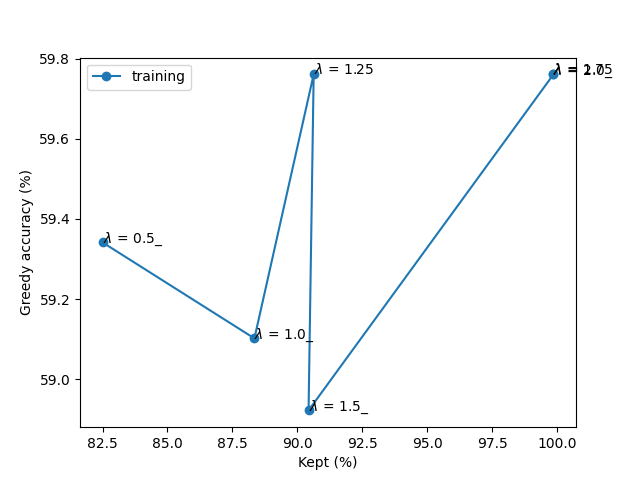
\includegraphics[width=1.1\textwidth]{figs/unstructured_acc_cost_train.png}
        \caption{Unstructured model, training set}
        \label{fig:unstr_train}
    \end{subfigure}
    \hfill
    \begin{subfigure}[b]{0.47\textwidth}
        \centering
        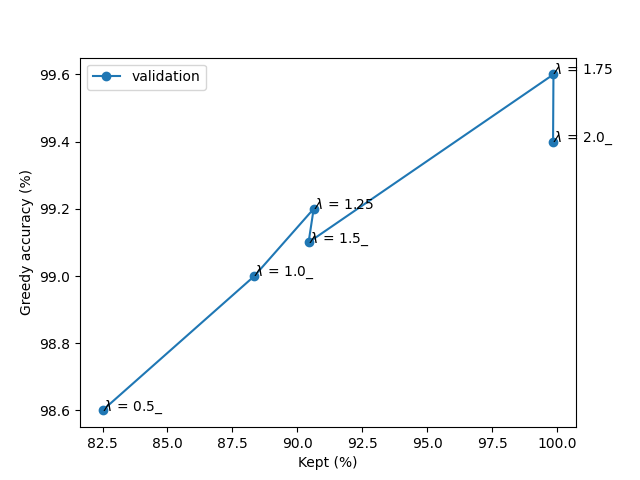
\includegraphics[width=1.1\textwidth]{figs/unstructured_acc_cost_val.png}
        \caption{Unstructured model, validation set}
        \label{fig:unstr_val}
    \end{subfigure}
    \hfill
    \begin{subfigure}[b]{0.47\textwidth}
        \centering
        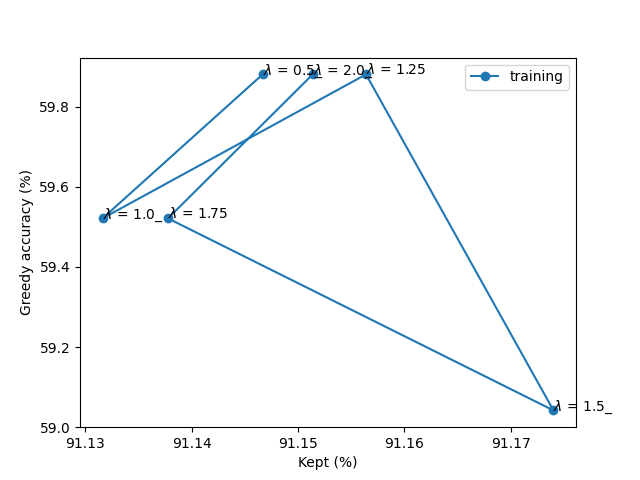
\includegraphics[width=1.1\textwidth]{figs/structured_acc_cost_train.png}
        \caption{Segmentation model, training set}
        \label{fig:str_train}
    \end{subfigure}
    \hfill
    \begin{subfigure}[b]{0.47\textwidth}
        \centering
        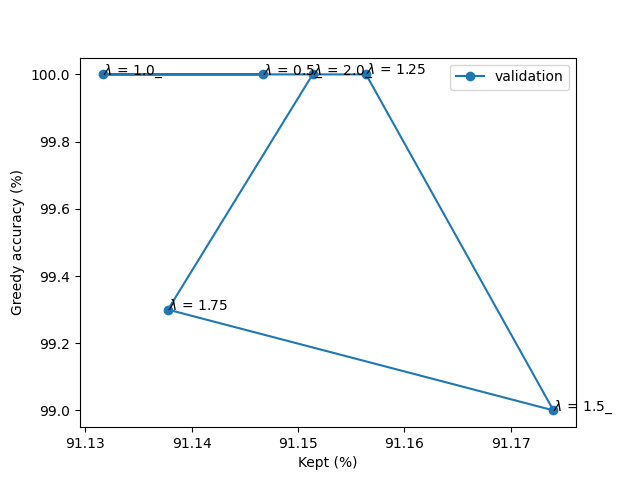
\includegraphics[width=1.1\textwidth]{figs/structured_acc_cost_val.png}
        \caption{Segmentation model, validation set}
        \label{fig:str_val}
    \end{subfigure}
    \caption{Accuracy and cost}
    \label{fig:acc_cost}
\end{figure}

\begin{figure}
    \centering
    \begin{subfigure}[b]{0.47\textwidth}
        \centering
        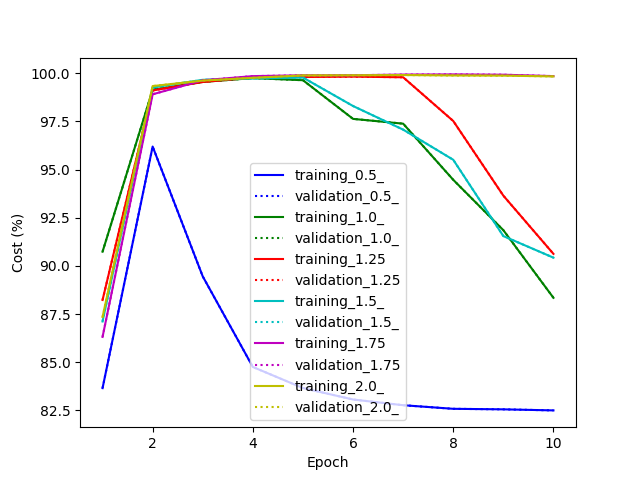
\includegraphics[width=1.1\textwidth]{figs/unstructured_cost.png}
        \caption{Unstructured model}
        \label{fig:unstr_cost}
    \end{subfigure}
    \hfill
    \begin{subfigure}[b]{0.47\textwidth}
        \centering
        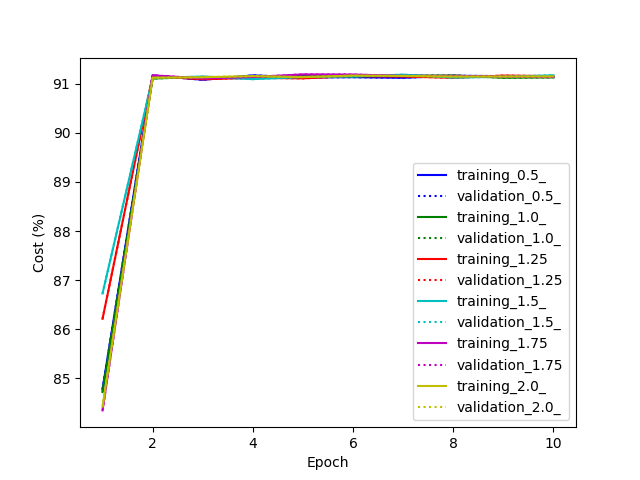
\includegraphics[width=1.1\textwidth]{figs/structured_cost.png}
        \caption{Structured model}
        \label{fig:str_cost}
    \end{subfigure}
    \caption{Cost}
    \label{fig:cost}
\end{figure}

\begin{figure}
    \centering
    \begin{subfigure}[b]{0.47\textwidth}
        \centering
        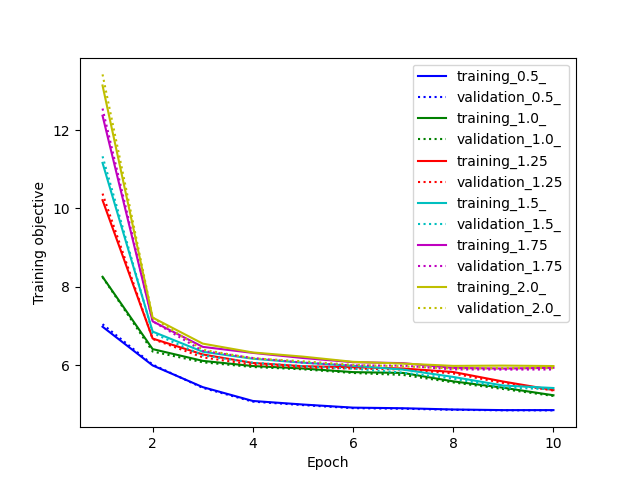
\includegraphics[width=1.1\textwidth]{figs/unstructured_obj.png}
        \caption{Unstructured model}
        \label{fig:unstr_obj}
    \end{subfigure}
    \hfill
    \begin{subfigure}[b]{0.47\textwidth}
        \centering
        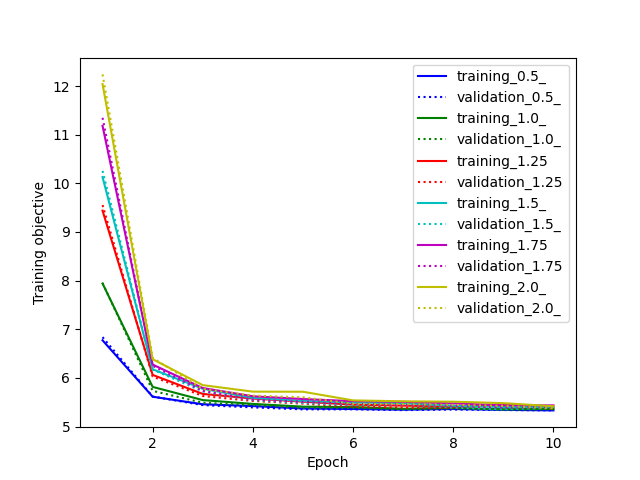
\includegraphics[width=1.1\textwidth]{figs/structured_obj.png}
        \caption{Structured model}
        \label{fig:str_obj}
    \end{subfigure}
    \caption{Training objective}
    \label{fig:obj}
\end{figure}

\begin{figure}
    \centering
    \begin{subfigure}[b]{0.47\textwidth}
        \centering
        \includegraphics[width=1.1\textwidth]{figs/high_acc_cost_val.png}
        \caption{Accuracy and cost}
        \label{fig:high_cost_acc}
    \end{subfigure}
    \hfill
    \begin{subfigure}[b]{0.47\textwidth}
        \centering
        \includegraphics[width=1.1\textwidth]{figs/high_cost_10000.png}
        \caption{Cost}
        \label{fig:high_cost}
    \end{subfigure}
    \hfill
    \begin{subfigure}[b]{0.47\textwidth}
        \centering
        \includegraphics[width=1.1\textwidth]{figs/high_obj_10000.png}
        \caption{Training objective}
        \label{fig:high_obj}
    \end{subfigure}
    \caption{Results with $\lambda = 10000$}
    \label{fig:high}
\end{figure}

\end{document}